\noindent The diagram seen in figure \ref{fig:Polite-Mobile-Obstacle-Avoidance-Flowchart} illustrates the software logic flow for our system. \\

\noindent The flowchart begins at processing the Sonar sensor readings. These readings are done first due to their relatively low latency and accuracy for determining if we are in need of an immediate stop.  \\

\begin{figure}[H]
	\centering
	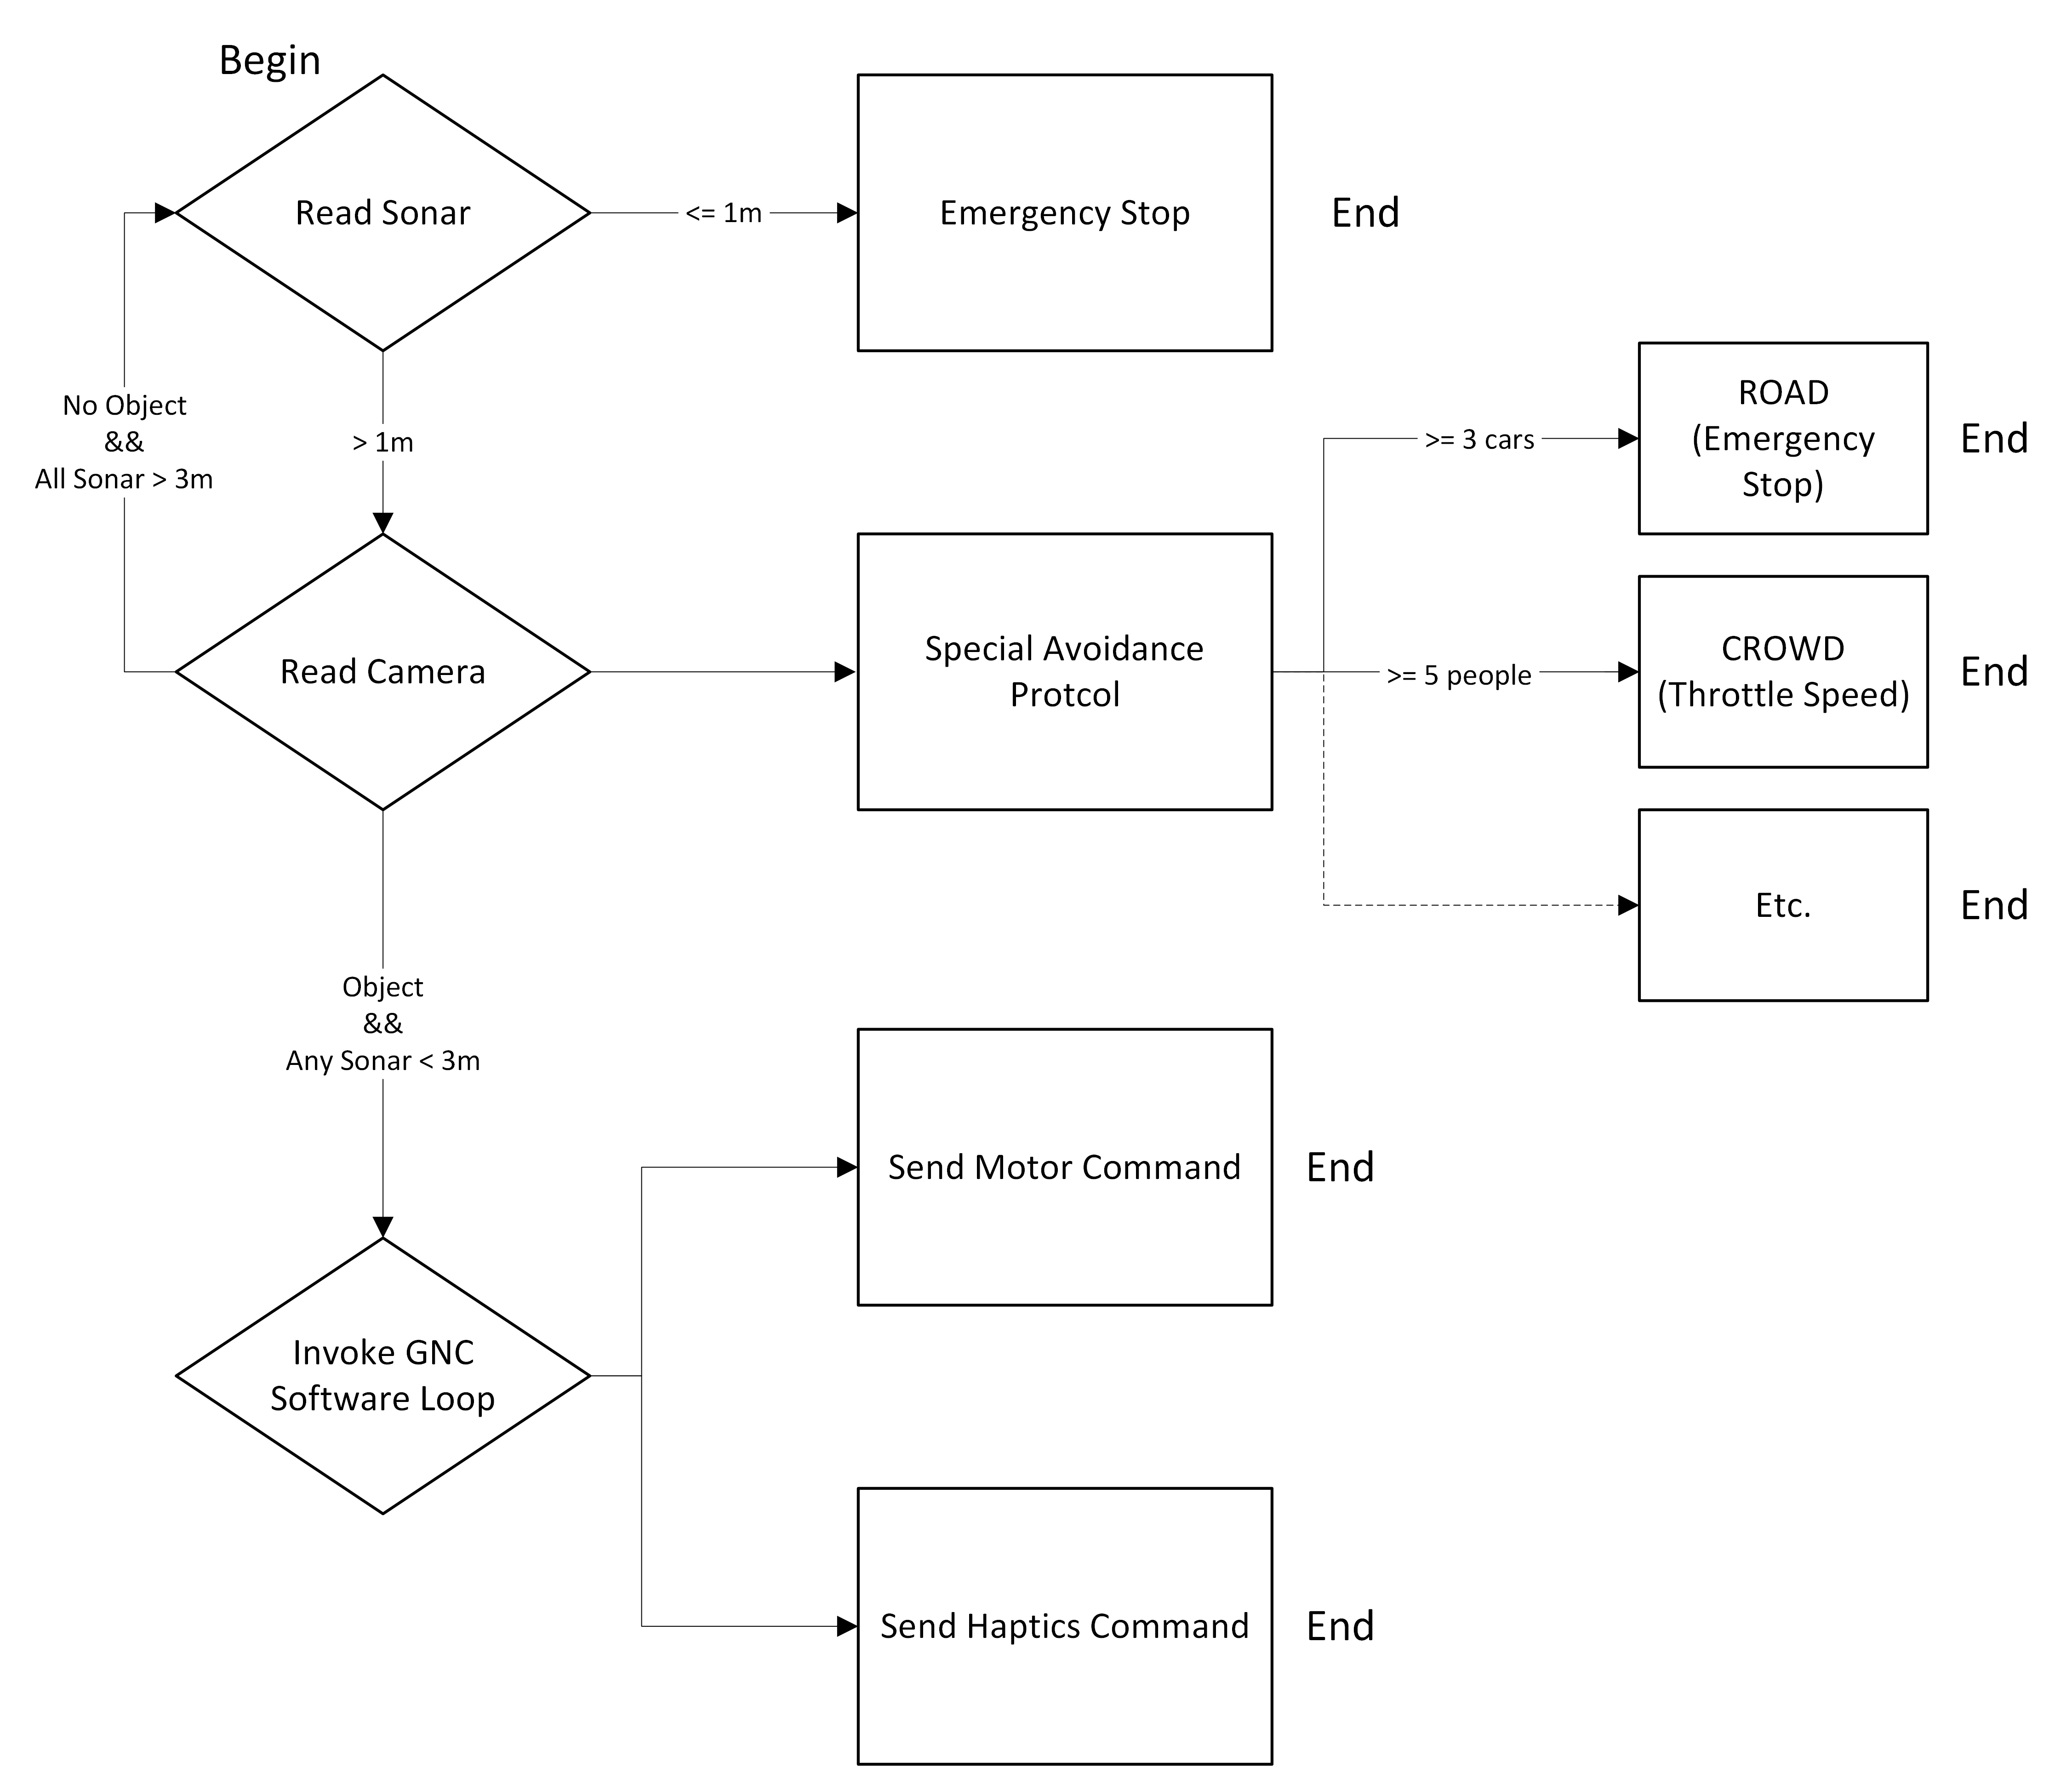
\includegraphics[width=1.0\textwidth]{./Images/Polite-Mobile-Obstacle-Avoidance-Flowchart.png}
	\caption{\label{fig:Polite-Mobile-Obstacle-Avoidance-Flowchart}Polite Mobile Obstacle Avoidance Flowchart}
\end{figure}

\subsection{Guidance, Navigation, and Control Software}
\noindent The block titled "invoke GNC software loop" seen in figure \ref{fig:Polite-Mobile-Obstacle-Avoidance-Flowchart} illustrates the softwre \\  does ... [TOBYBOT GET IN HERE CHIEF KEEF] \\


\noindent GNC situation, tilt (attitude) using IMU, (incline decline), velocity and position solutions, ESP32 source code GitHub (hc-sr04.c luna.c haptic.c audio.c motor.c ip.c avoid.c), motor commands calculation. \\


\subsection{Object Detection}
\noindent The computer vision aspect of our software is very straight forward. The Arduino IDE contains example code for each board file and has an example of an object detection algorithm for the AMB-82 board. To implement this for our purposes, we maintained the YOLO4 Tiny model configuration, the already existing class list for the objects to be detected, and the main loop to extract this data from the algorithm. \\

\noindent While we were able to utilize the example code to help in getting started, there was additional functionality needed to properly fit our purposes. The first of these was implementing WiFi and UDP communication on the board. After doing such, we used a while loop to wait for the ESP32 to assert a transmit flag and once received, the AMB-82 board would complete an object detection run and transmit the data to the ESP32. \\

\subsection{Computer Vision}
\noindent \textit{Classify grass by green color!}


\subsection{Serial Interfaces}
\noindent As discussed in section \ref{ardumatlab}, we can port the serial plotter data for the ranges and IMU to MATLAB in order to visualize the field of view. See equation \ref{Polar}. We can visualize obstacles present because of dips in the range outputs. We also can visualize attitude and orientation based on IMU outputs. Putting these into MATLAB plots will provide valuable insight into the dynamics of the entire system as it traverses a test environment. It also interfaces between non-visual and visually based sensing methods by creating a map of the environment.\\

\noindent Mathematically, we know that the \underline{\textit{navigational plane}} is two-dimensional, with the reference frame origin located at the rollator center of mass. The positive x-axis is forward looking aft, the positive y-axis is left facing aft, and the positive z-axis is vertically upward. Because of the 2D nature, we can negate the z-axis because we do not sense altitude, nor is FORWARD an airborne system. It always stays grounded. Therefore, the guidance commands are given to the yaw angle (x-axis orientation) and the motor speed, which is actuated when on an incline or decline as shown in \ref{fig:slope-stability}. In essence, based on obstacles detected and classified, FORWARD will prompt the user to steer left or right. It should never prompt the user to go backwards or to travel vertically upward. The one exception is for curb lifting, which admittedly is a difficult maneuver to achieve: a stretch goal.\\

\subsection{Motor Control Software}


\noindent [UML CLASS DIAGRAM HERE]\\